%% 
%% Copyright 2007-2020 Elsevier Ltd
%% 
%% This file is part of the 'Elsarticle Bundle'.
%% ---------------------------------------------
%% 
%% It may be distributed under the conditions of the LaTeX Project Public
%% License, either version 1.2 of this license or (at your option) any
%% later version.  The latest version of this license is in
%%    http://www.latex-project.org/lppl.txt
%% and version 1.2 or later is part of all distributions of LaTeX
%% version 1999/12/01 or later.
%% 
%% The list of all files belonging to the 'Elsarticle Bundle' is
%% given in the file `manifest.txt'.
%% 

%% Template article for Elsevier's document class `elsarticle'
%% with numbered style bibliographic references
%% SP 2008/03/01
%%
%% 
%%
%% $Id: elsarticle-template-num.tex 190 2020-11-23 11:12:32Z rishi $
%%
%%
\documentclass[preprint,12pt]{elsarticle}

%% Use the option review to obtain double line spacing
%% \documentclass[authoryear,preprint,review,12pt]{elsarticle}

%% Use the options 1p,twocolumn; 3p; 3p,twocolumn; 5p; or 5p,twocolumn
%% for a journal layout:
%% \documentclass[final,1p,times]{elsarticle}
%% \documentclass[final,1p,times,twocolumn]{elsarticle}
%% \documentclass[final,3p,times]{elsarticle}
%% \documentclass[final,3p,times,twocolumn]{elsarticle}
%% \documentclass[final,5p,times]{elsarticle}
%% \documentclass[final,5p,times,twocolumn]{elsarticle}

%% For including figures, graphicx.sty has been loaded in
%% elsarticle.cls. If you prefer to use the old commands
%% please give \usepackage{epsfig}

%% The amssymb package provides various useful mathematical symbols
\usepackage{amssymb}
%% The amsthm package provides extended theorem environments
%% \usepackage{amsthm}

%% The lineno packages adds line numbers. Start line numbering with
%% \begin{linenumbers}, end it with \end{linenumbers}. Or switch it on
%% for the whole article with \linenumbers.
%% \usepackage{lineno}

\usepackage{xcolor}
\usepackage{soul}
\newcommand{\hly}[2][yellow]{{
  \colorlet{foo}{#1}
  \sethlcolor{foo}\hl{#2}}
}
\newcommand{\hlr}[2][red]{{
  \colorlet{foo}{#1}
  \sethlcolor{foo}\hl{#2}}
}
\newcommand{\hlg}[2][green]{{
  \colorlet{foo}{#1}
  \sethlcolor{foo}\hl{#2}}
}
\newcommand{\hlo}[2][orange]{{
  \colorlet{foo}{#1}
  \sethlcolor{foo}\hl{#2}}
}
\newcommand{\hlb}[2][brown]{{
  \colorlet{foo}{#1}
  \sethlcolor{foo}\hl{#2}}
}
\newcommand{\hlgr}[2][lightgray]{{
  \colorlet{foo}{#1}
  \sethlcolor{foo}\hl{#2}}
}

\journal{Lancet Public Health}

\begin{document}

\begin{frontmatter}

%% Title, authors and addresses

%% use the tnoteref command within \title for footnotes;
%% use the tnotetext command for theassociated footnote;
%% use the fnref command within \author or \address for footnotes;
%% use the fntext command for theassociated footnote;
%% use the corref command within \author for corresponding author footnotes;
%% use the cortext command for theassociated footnote;
%% use the ead command for the email address,
%% and the form \ead[url] for the home page:
%% \title{Title\tnoteref{label1}}
%% \tnotetext[label1]{}
%% \author{Name\corref{cor1}\fnref{label2}}
%% \ead{email address}
%% \ead[url]{home page}
%% \fntext[label2]{}
%% \cortext[cor1]{}
%% \affiliation{organization={},
%%             addressline={},
%%             city={},
%%             postcode={},
%%             state={},
%%             country={}}
%% \fntext[label3]{}

\title{How city design contributes to changes in mode choice and health risks during a crisis: a global observational study}

%% use optional labels to link authors explicitly to addresses:
%% \author[label1,label2]{}
%% \affiliation[label1]{organization={},
%%             addressline={},
%%             city={},
%%             postcode={},
%%             state={},
%%             country={}}
%%
%% \affiliation[label2]{organization={},
%%             addressline={},
%%             city={},
%%             postcode={},
%%             state={},
%%             country={}}

\author[melb]{Kerry~A.~Nice\corref{cor1}}
\author[melb]{Jason Thompson}
\author[melb]{Belen Zapata-Diomedi}
\author[melb]{Leandro Garcia}
\author[melb]{Haifeng Zhao}
\author[melb]{Sachith Seneviratne}
\author[melb]{Ruth Hunter}
\author[melb]{Rodrigo Siqueira Reis}
\author[melb]{Mark Stevenson}
\author[melb]{et al.}

\cortext[cor1]{Principal corresponding author}
\ead{kerry.nice@unimelb.edu.au}
\address[melb]{Transport, Health, and Urban Design Research Lab, Faculty of Architecture, Building, and Planning, University of Melbourne, VIC, Australia.}
%\address[eng]{Melbourne School of Engineering; and Melbourne School of Population and Global Health, University of Melbourne, VIC, Australia.}

%\affiliation{organization={},%Department and Organization
%            addressline={}, 
%            city={},
%            postcode={}, 
%            state={},
%            country={}}

%\begin{abstract}
%% Text of abstract

%\end{abstract}

%%Graphical abstract
%\begin{graphicalabstract}
%\includegraphics{grabs}
%\end{graphicalabstract}

%%Research highlights
%\begin{highlights}
%\item Research highlight 1
%\item Research highlight 2
%\end{highlights}

%\begin{keyword}
%% keywords here, in the form: keyword \sep keyword

%% PACS codes here, in the form: \PACS code \sep code

%% MSC codes here, in the form: \MSC code \sep code
%% or \MSC[2008] code \sep code (2000 is the default)

%\end{keyword}

\end{frontmatter}

%% \linenumbers

%% main text

\section*{Introduction}

City designs are highly influenced by the dominant transport modes present at the time of their development \cite{KNOWLES2020102607}. The designs which vary within and between cities, form a scaffold upon which citizens move and interact \cite{Thompson2020}. City designs therefore both afford and constrain transport mode choice and signifcantly influence mobility patterns, which influence lifestyles and exposure to health risks. \cite{WHO2023}.

The design of cities arise from either a  strict top-down planning regime \cite{mundigo1977city} or organically through bottom-up processes \cite{batty2017thinking}. While some city designs foster movement and patterns of interaction that reduce exposure to significant health risks including air pollution, physical inactivity and the concomitant chronic diseases\cite{Wijnands2022, Stevenson2016,wang2023flood, stanley2022managing}. Given that approximately 56 percent of the world's 8 billion population live in cities — with projections it will reach 68 percent by 2050 \cite{WHO2023} understanding the role of city design in an effort to mitigate and prevent adverse health outcomes is of paramount importance in efforts to reduce the global burden of disease. 

Accessing data that is standardised and readily accessible is urgently needed in order to explore city designs and the role that city design plays in mitigating or exacerbating health risks. Accessing the necessary data is a challenge given the majority of globally available data sources at the level of the city, are held in the Global North, while the majority of the world's urban population lives in the Global South \cite{Smit2021}.

Clear evidence now underlines how public health risks encompassing injury, overweight, obesity, mental illness, respiratory disease, and other health issues entwined with inequality and social disadvantage are entrenched in the fabric of city designs, whether planned or otherwise \cite{borrell2013factors,xing2016impact,yuchi2020road}. Not all cities nor parts of cities are on equal footing when faced with public health threats and hazards, rendering some citizens - usually the most disadvantaged - at greater risk of ill-health \cite{KRISHNA2021102046}. For example, both social inequity brought about through road and highway construction \cite{carpenter2010poverty,archer2020white} and the burden of disease attributable to road transport-related air pollution disproportionately affects poorer communities who live close to major roadways, as well as children and the elderly. Air pollution-related deaths peak among babies in the early (0-6 days) and late (7-27 days) neonatal groups, reflecting how particulate matter can cause lower-respiratory infections in new-borns. These deaths then peak again in older age groups, as air pollution contributes to lower-respiratory infections as well as noncommunicable diseases that develop over time, such as ischaemic heart disease, stroke, COPD, and lung cancer \cite{boogaard2022long}. 

Similarly, rates of road trauma are disproportionately high in both cities and areas within cities where exposure to risk (i.e., through use of and interaction with motor-vehicles) is greatest. Previous work has demonstrated that the per-capita burden of road transport injury for the poorest-performing global city types is an estimated 2-times greater than the best performing city types, producing an estimated loss of nearly 9 million disability-adjusted life-years attributable to sub-optimal urban design per annum \cite{Thompson2020}. Similarly, differences in road and intersection design within cities can produce considerable variation in risk exposure for residents \cite{Wijnands_IntersectionDesign2021,MORRISON2019123}. Such elevated risk is in addition to that generated through auto-centric urban design that disproportionately forces car use and ownership upon already disadvantaged households \cite{currie2018alarming, CURL201861}. 

However, the evolution and dynamics of cities also generates dynamic risk profiles where risk exposure can shift dramatically in response to unfolding and overlapping events. For instance, cities with appropriate housing stock (e.g., large), industrial profile (e.g., service economy), demographic profile (e.g., nuclear families), and associated urban infrastructure (e.g., fast, widespread internet connection) may be well-suited to rapid adaptation to population-wide stay-in place policies \cite{hale2021global} triggered by biological or natural hazards. However, these population-wide policies may still place long-term economic burden on people who remain in manual jobs or in roles that cannot be performed remotely \cite{CraigWFH,Vyas2021}. This can heighten inequalities for already vulnerable and high-risk communities \cite{martin2020fighting} which may in-turn foster resentment and resistance toward observance of public health interventions \cite{de2016sustainability}. When high-risk groups reject public health guidance, risk to the general population is elevated, especially in relation to communicable disease \cite{koopman2005control}.

Such intertwined scenarios highlight that cities are complex systems \cite{DiezRoux2015}, interventions are unlikely to be felt equally across all levels of society, and any solutions to crises or problems at hand are likely to set in motion a chain of secondary effects whose outcomes may or may not be well-understood at the outset \cite{Sterman2006}. When urban planning regimes and city designs meet mass public health challenges and interventions that impact populations and unfold over varying time-scales \cite{casti2012x}, they pose significant planning, management, and communication challenges for policymakers \cite{thompson2022modelling,thompson2022framework}. Hence, public health interventions demand a nuanced understanding of both long-term and short-term societal outcomes, population heterogeneity, public health trade-offs, and the likely time-frames within which they may prove effective, accepted and/or justified in the context of the city in which they are enacted \cite{dawson2016snakes, oliu2021sars}.


\textbf{Objectives}

The objective of this manuscript is to describe how city designs influenced changes to travel patterns and mode share between public versus private transportation during the first year of the CoVID-19 pandemic. We set out to evaluate the changes in transport-related pollution levels (namely, \(PM_{2.5}\) and \(NO_{2}\)) and exposure to transport injury risk across each of 639 cities, worldwide. We seek to demonstrate how estimated population health outcomes across respiratory disease, road injuries, and infectious disease are associated with differences in urban design characteristics across global cities.

Our aim is to illustrate how different city designs both afford and/or constrain the ability of cities and their populations to adapt to and recover from crises such as the CoVID-19 pandemic. We discuss the implications of our findings for future public health challenges that cities and populations around the world will face in the future. Our final objective is to identify which urban design types might demonstrate the greatest resilience against likely immediate and long-term global public health threats. 


\textbf{Main research question}

 Which global city designs demonstrate the greatest resilience to both acute and chronic health challenges?


% \section*{Research in context}

% \textbf{Evidence before this study} 
% A paragraph about what existed before.

% \textbf{Added value of this study} 
% A paragraph about what the study provides.

% \textbf{Implications of all the available evidence} 
% A paragraph about the implications of the study.



\section*{Methods}



\subsection*{Data analysis}
The initial step of this research was to create a representation of cities that accurately captured important features of urban design related to mobility and public health. To accomplish this, a graph neural network was constructed, utilising OpenStreetMap road network data (nodes and edges) as input from each of 1632 global cities previously identified in \cite{Thompson2020}. Graph neural networks work by forming high-dimensional hypotheses that can effectively represent the data input into them; in this case, road networks, public transit networks, and active transport networks (e.g., walking and cycling paths) derived from OpenStreetMap data\cite{Boeing2017a}. In the context of understanding mobility patterns, the utilisation of OpenStreetMap data offers significant advantages over sampled imagery data used in previous studies (e.g., \cite{Thompson2020,seneviratne2021self}) due to OpenStreetMap data's high density and its capacity to represent features of an entire city, rather than relying upon sampled data from locations across cities. Furthermore, in comparison to the use of imagery data, the analysed road networks of each city present a direct, rather than inferred data source relating to mobility and urban form. The cities used in this analysis are depicted in Figure \ref{fig:clusters}.


\begin{figure}
\centering
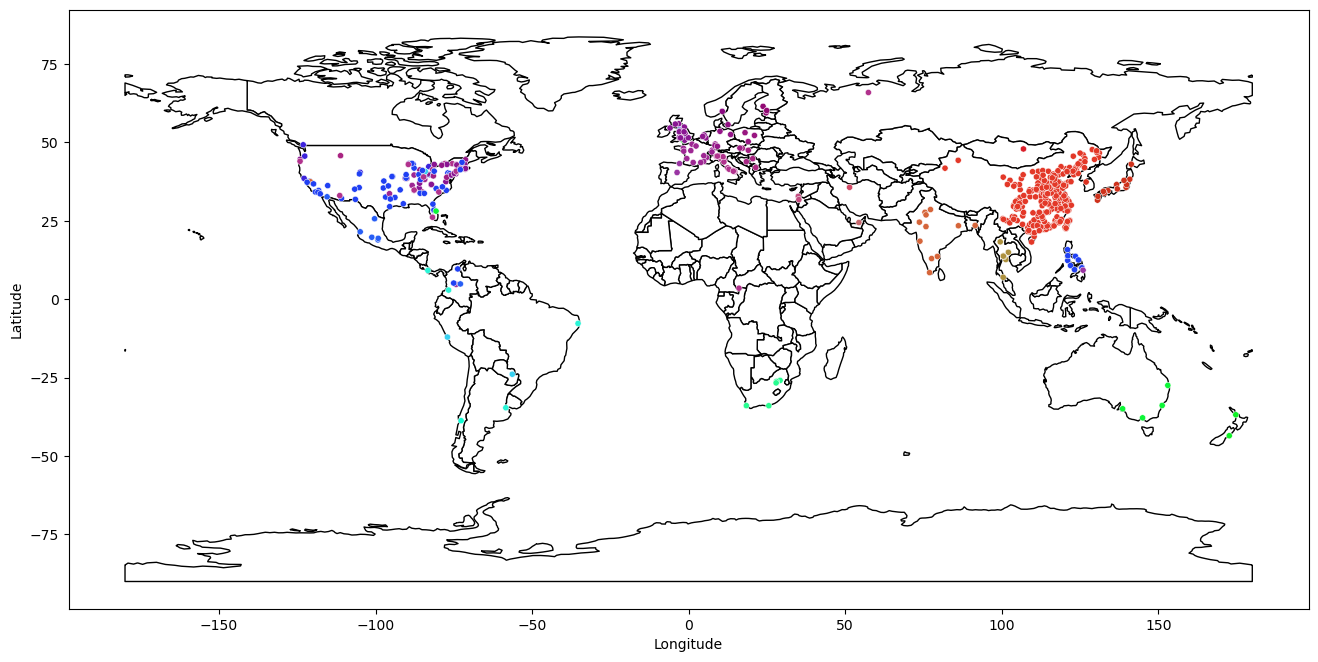
\includegraphics[trim={0 0 0 0},clip,scale=0.4]{Images/ByCountry_map_Zeigler.png}
\caption{\bf Location of the 679 cities used in this study.}
 \label{fig:clusters}
\end{figure}


The graph neural network was trained using self-supervised learning; a method proven to capture urban form comparably to supervised learning \cite{seneviratne2021self}. Importantly, this allows the graph neural network used here to represent the data without requiring a labelled output to the neural network (such as city names used in \cite{Thompson2020}).

Masked Auto-encoding (MAE) was used as the training objective of the graph neural network. This objective has demonstrated effective performance in neural networks across various data modalities such as graphs\cite{hou2022graphmae}, images\cite{he2022masked} and text\cite{devlin2018bert}. MAE trains the neural network by `masking' part of the input data, then tasking the model with predicting the masked (unknown) portion. Here, we masked both road (edge) features - such as length, start and end locations of roads - as well as node features such as latitude and longitude. The model then attempted to predict surrounding OpenStreetMap sections from the remainder of the available sample. 

The results of this analysis were then converted to a t-SNE graph which organised the average value of each city OpenStreetMap sample in a 2-dimensional plane where the distance between cities on the graph represented their similarities across urban characteristics (see Figure \ref{fig:tSNE}).

City-level pollution data was employed to validate the representation learned by the neural network. For each city, the neural network could predict whether pollution levels rose or fell compared to the previous year with an accuracy of 97\%. This result underscores the neural network's ability to not only capture the road network of the modelled cities, but also to approximate the relationship between the transport network and the behaviour of pollutants within the city.

Additional validation of the neural network comes from Figure \ref{fig:Dimensions}, which plots the t-SNE representation against understood dimensions of urban design measured against city block size, block regularity, and block number as well as percentage of road and transit networks observed in each city from prior studies \cite{Thompson2020}. Combined with Figure \ref{fig:clusters} and Figure \ref{fig:tSNE}, Figure \ref{fig:Dimensions} demonstrates that the urban morphology for analysed cities follows gradual changes across dimensions. High-density, small-block size and relatively regular cities are depicted on the upper-left of the chart (e.g., in areas A1/A2 and B1/B2), whereas sparse, large-block cities with little public transit infrastructure as a proportion of the transport network cluster together in the bottom right through areas G7 to H7. 

Figure \ref{fig:tSNE} also shows that cities from within countries and continents tend to cluster together. For example, Japanese cities cluster tightly together across areas A1 and B1, while European cities cluster together in and around areas A2 to B2. Asian cities across China, India and Vietnam extend in a regular pattern from grid references B3 through to H7 as their designs differed along dimensions of block size and road network density.

Of note are also clusters of Australasian, South American and North American cities found in areas A3 to A5 and B3 to B5. Urban designs in these areas tended to demonstrate regular, medium-sized blocks with medium to low levels of public transit. Cities in these locations were typically of a `Chequerboard' or `Motor City' types, designed to facilitate the egress of motor vehicles.

\begin{figure}
\centering
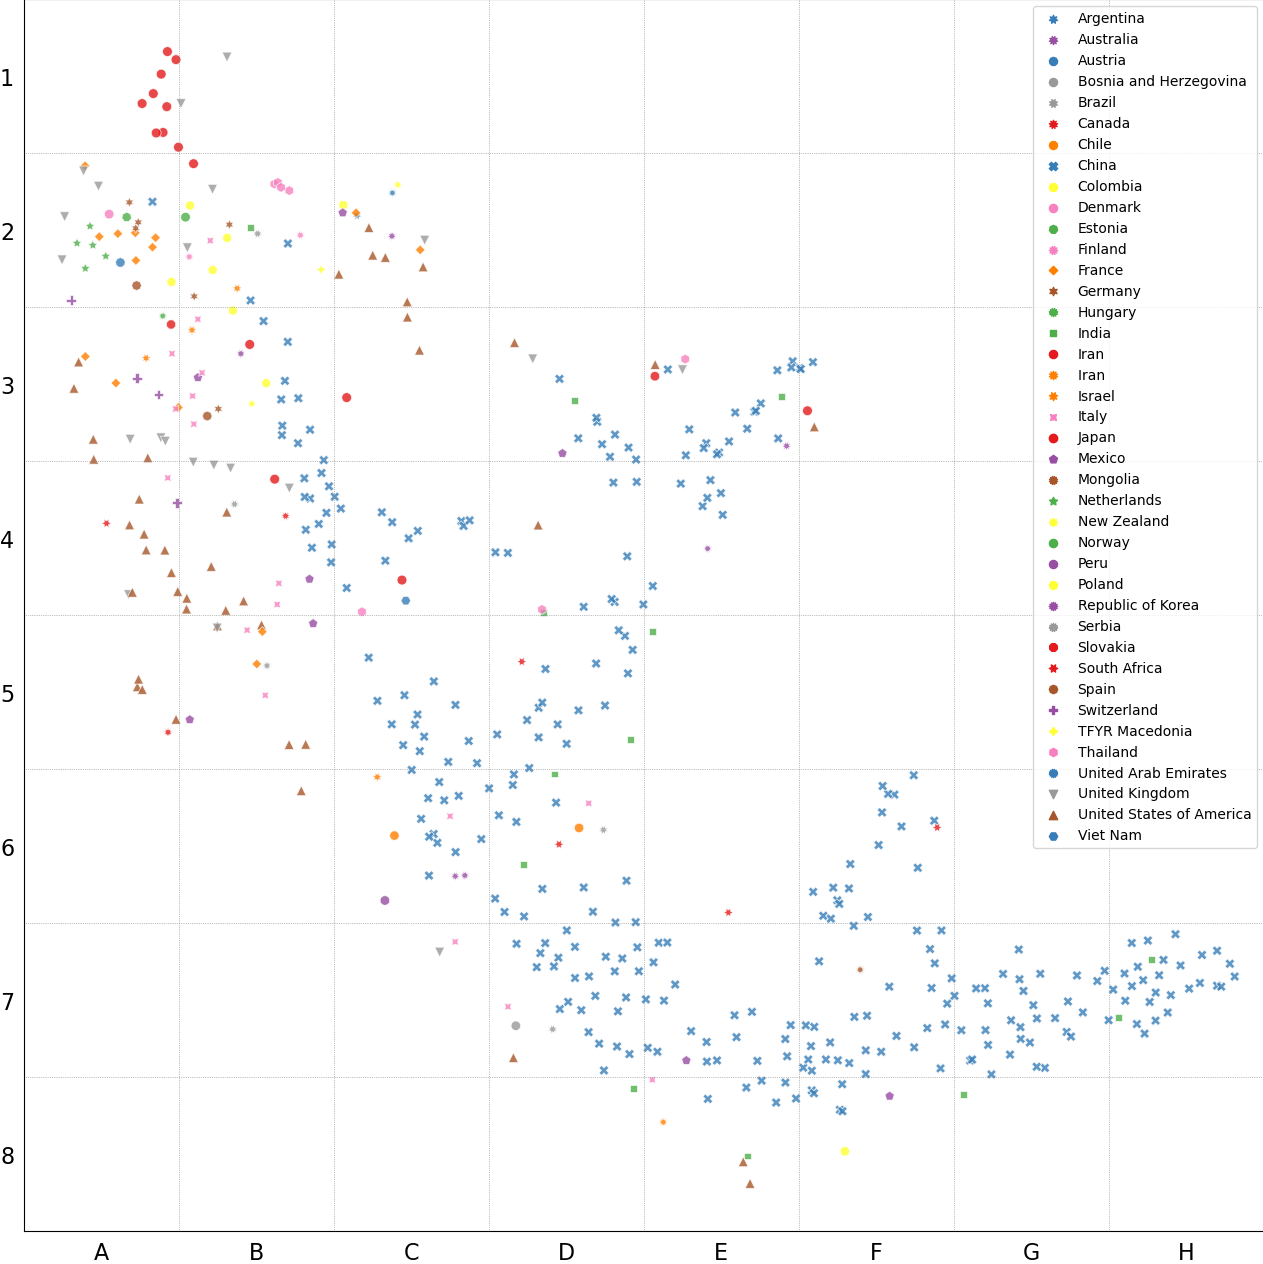
\includegraphics[trim={ 0 0 0 0 },clip,scale=0.45]{Images/tSNE Country.png}
\caption{\bf 2-dimensional, t-SNE representation of all modelled cities in the analysis.}
 \label{fig:tSNE}
\end{figure}


\begin{figure}
\centering
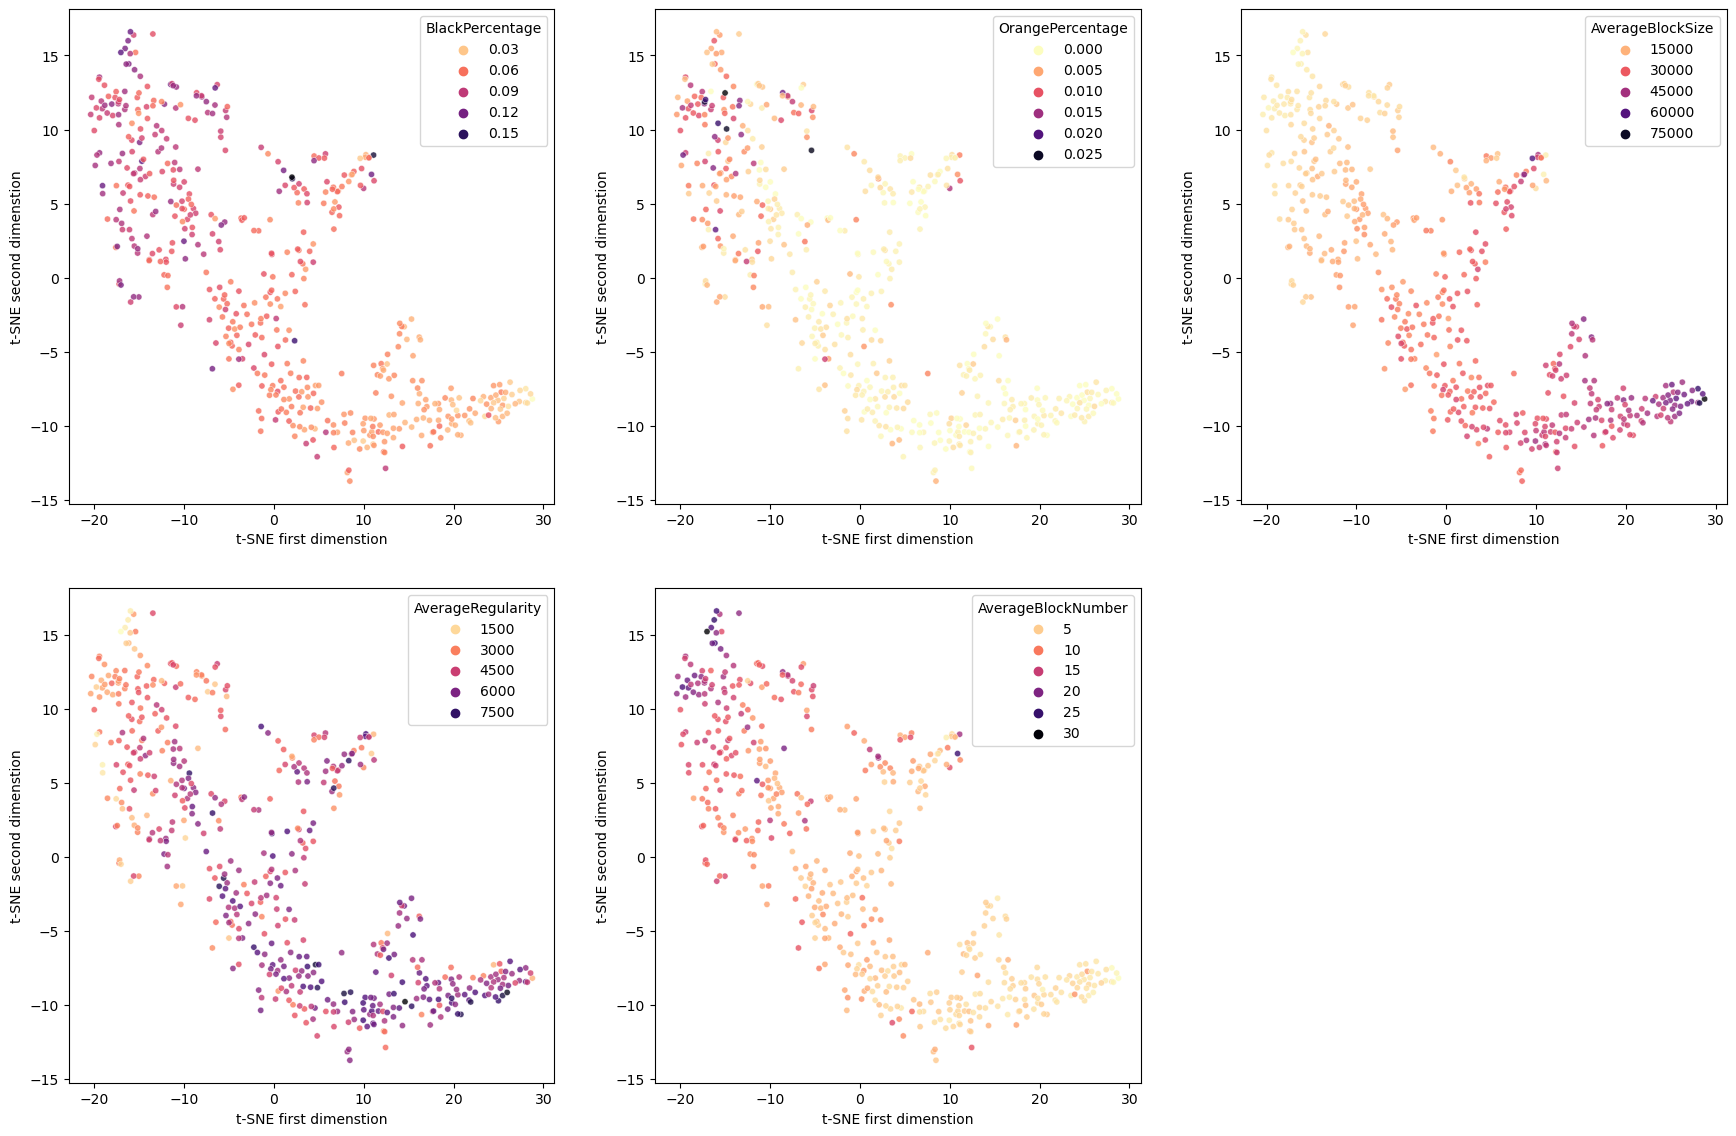
\includegraphics[trim={ 0 0 0 0 },clip,scale=0.35]{Images/City Types Dimensions.png}
\caption{\bf 2-dimensional, t-SNE representation of all modelled cities in the analysis.}
 \label{fig:Dimensions}
\end{figure}




\subsection*{Data sources}


Wijnands et al. (2022) \cite{Wijnands2022} created pollutant and city specific XGBoost models for 679 cities, trained on weather and pollution observations over 2015-2019 and used these models to predict daily pollution levels of NO$_{2}$, PM$_{2.5}$, PM$_{10}$, and O$_{3}$ during 2020. Using 2020 observed values, anomalies were calculated in the absence of a pandemic. The original Thompson et al. (2020)\cite{Thompson2020} urban typology dataset consisted of the largest 1632 cities in the world. Of these, a subset of 679 cities were used (see Figure \ref{fig:clusters}), those that had pollution data available.

Apple \cite{Apple2020} and Google \cite{Google2020} provided mobility indexes in 2020. Apple's index calculates differences in map requests for modes of walking, driving, or public transit over a January 2020 baseline. Google generated an index using phone-tracking-based changes in mobility across several types of locations, including retail and recreation, grocery stores and pharmacies, parks, transit stations, workplaces, and private residences. These daily indexes were linked to the 679 cities with available pollution data.

Google's COVID-19 Open Data repository \cite{Google2022} provides data for daily COVID-19 cases using a consistent set of region keys. Daily values were linked to the 679 cities when city case data was available, matching country-level to cities when city-level data was unavailable.


%\textbf{Stringency: } Oxford COVID-19 Government Response Tracker. The baseline measure of variation in governments' responses is the COVID-19 Government Response Stringency Index. This composite measure is a simple additive score of the seven indicators (S1-S7) measured on an ordinal scale, rescaled to vary from 0 to 100. https://covidtracker.bsg.ox.ac.uk/







\begin{figure}
\centering
%\fbox{
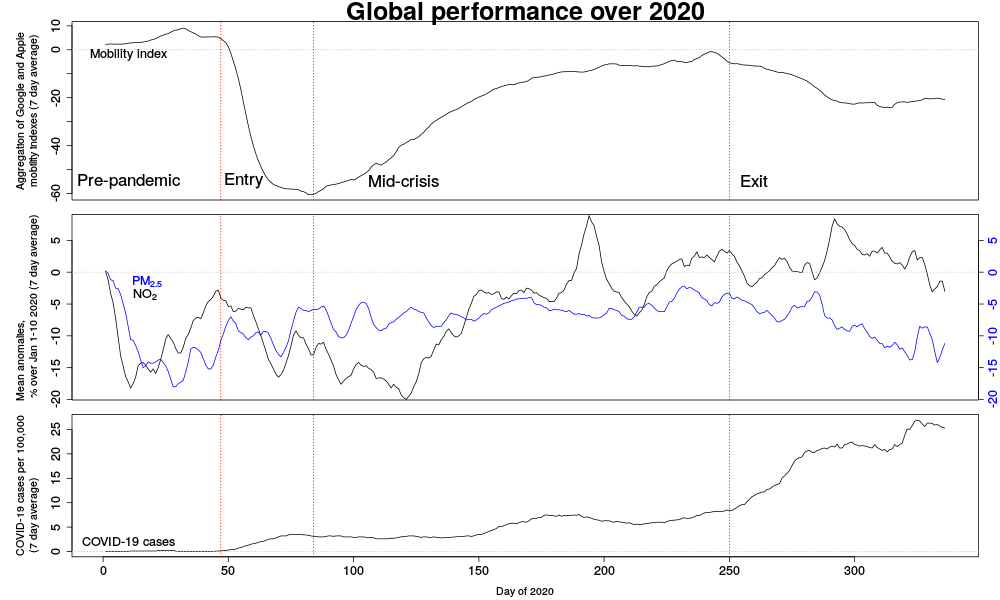
\includegraphics[trim={0 0 15 20},clip,scale=0.45]{Images/LancetPHOverall.png}
%}
\caption{\bf Overview of COVID-19 crisis progression and stages across 679 global cities over 2020. Seven day rolling average aggregations of Google and Apple mobility indexes (top), seven day rolling averages of pollution percentage anomalies over January 1-10, 2020 baseline (middle), and seven day rolling average COVID-19 cases per 100k (bottom). This figure will be replaced, but just keeping it here for the moment to demonstrate overall trends}
 \label{fig:stages}
\end{figure}

\section*{Results}

\begin{figure}
\centering
%\fbox{
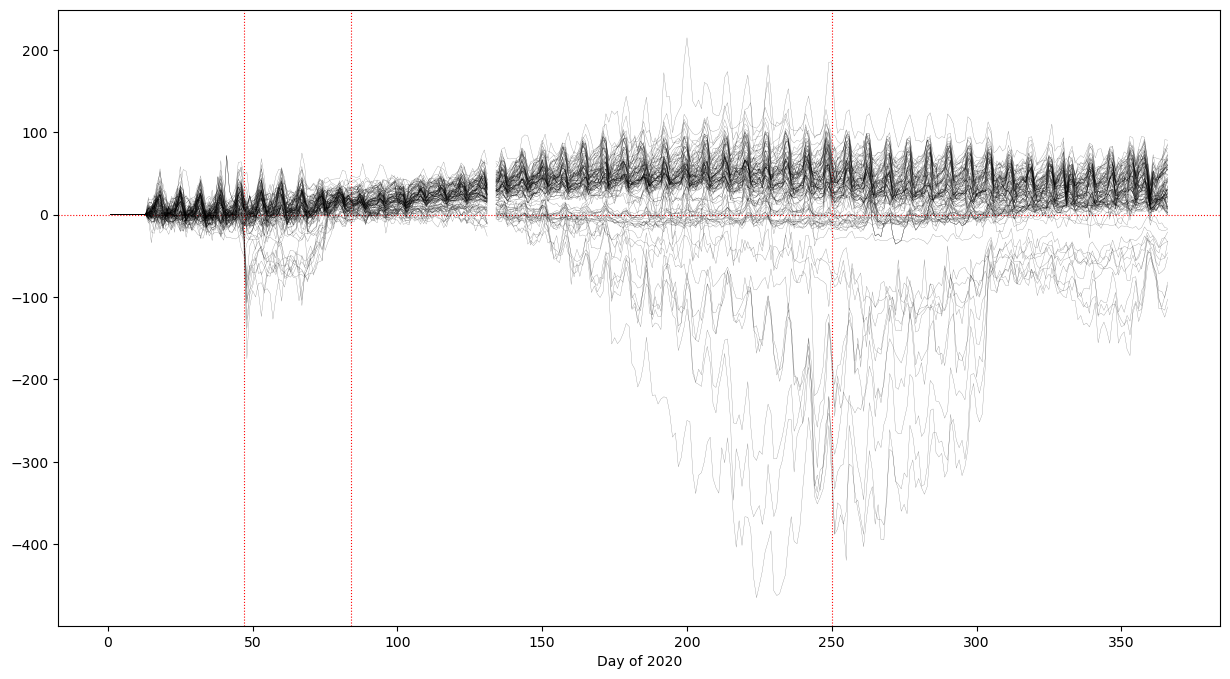
\includegraphics[trim={0 0 0 0},clip,scale=0.4]{Images/DrivingvsTransit.png}
%}
\caption{\bf An overview of observed modal shift from public transit to private motor vehicles observed during 2020 for all analysed cities highlighting an increased reliance on private vehicle use over public transit during during the course of the COVID-19 pandemic. Values \textgreater 0 indicate a proportional replacement of public transit trips to private vehicles for individual cities in comparison to pre-pandemic conditions.}  
 \label{fig:driv_trans}
\end{figure}


Figure \ref{fig:stages} shows average mobility (Panel 1), anomalies of NO$_{2}$ and PM$_{2.5}$ pollution levels (Panel 2), and total reported CoVID-19 cases (Panel 3) for all measured cities during 2020 across the `Pre-pandemic', `Entry', `Mid-Crisis', and `Recovery' phases of the CoVID-19 pandemic defined as between between days 0 and 46, 47 to 75, 76 to 250 and day 251+, respectively. Mobility measures are calculated as seven day rolling average aggregations of Google and Apple across the 679 cities for which data was available across both mobility and pollution. Pollution anomalies are calculated as percentage seven day rolling average differences over a January 1-10, 2020 baseline. CoVID-19 cases are calculated as a 7-day rolling average of cases per 100,000 population from \cite{Google2022}.

From Figure \ref{fig:stages} it is possible to observe the dramatic impact on global mobility that resulted from the introduction of movement restrictions, including stay-at-home orders, implemented across global cities during the pandemic's `Entry' phase \cite{hale2021global}. Although movement restrictions were designed as a public health measure to reduce person-to-person disease transmission, a secondary effect was that they led to significant reductions in mean transport-related NO$_{2}$ and PM$_{2.5}$ levels \cite{zhang2023impact}. Average mobility declined across cities, reaching a nadir at approximately 45 days after pandemic onset. This period also coincided with a plateau in global COVID-19 infection growth (panel 3) not least because of the public observance of mobility restrictions as well as other non-pharmaceutical interventions implemented up to and including this time \cite{hale2021global}. 

The mean estimated reduction in global NO$_{2}$ and PM$_{2.5}$ levels across observed cities during this `Entry' to `Mid-crisis' period was xxx\% or xxx ug/m$^{3}$. This equates to a cumulative reduction in pollution-related respiratory disease of xxx and a reduction in transport-related crash risk of yyy across analysed cities.

Alongside private vehicle transport, public transit ridership also declined by up to 90\% in the 'Entry' phase \cite{TransitCovid_Gkiotsalitis}. However, as mobility restrictions eased in response to declining rates of CoVID-19 transmission and populations began re-engaging with workplaces and social settings, citizens were faced with new factors that influenced their transportation choices including the risk of infection through the use of mass transit \cite{BECKTransit}. Figure \ref{fig:driv_trans}, shows how these concerns may have contributed to a global shift away from public transport ridership toward private vehicle use with values \textgreater 0 indicating a proportional modal shift away from public transit and toward private vehicle use. This trend across the vast majority of cities was most evident during July and August 2020, but continued until early 2021 with many cities implementing incentive programs to counteract the effect \cite{dai2021improving}.

Examining panel 3 of Figure \ref{fig:stages}, it is clear that the timing of the increase in private vehicle transport in mid-2020 coincided with a significant rebound of NO$_{2}$ and PM$_{2.5}$ levels than would be typically expected, adjusting for the weather, seasonality and trends, distinct topography, urban morphology, climate and atmospheric conditions of each city \cite{Wijnands2022}. This rebound was particularly pronounced for NO$_{2}$, which consistently exceeded estimated pre-pandemic levels across many cities in the latter part of 2020.

However, despite the global trend of transitioning from public transit to private motor vehicle use \cite{fernando2023shaping}, our results reveal that the extent of this shift was not uniform across all city types. Instead, it was more pronounced in cities recognised as being largely designed for motor vehicles \cite{Thompson2020} represented in areas A3 to A5 and B3 to B5 of Figure \ref{fig:tSNE}.

Characteristic designs of cities designed to promote the egress of motor vehicles is that they have planned, regular block layouts (for instance, square or rectangular block patterns) and have blocks of medium-size in comparison to other global cities \cite{Thompson2020}. Such vehicle-centric city designs are predominantly found in countries including the United States, Australia, Canada, New Zealand, and Argentina which have seen rapid urban expansion in the late 19th and early 20th centuries. During the pandemic's 'Mid Crisis' and 'Recovery' phases, the cities optimised for private vehicle transport afforded citizens a choice between public transit and private vehicle use. Given the public's fear of potential infectious disease transmission on public transit\cite{fernando2023shaping}, citizens who had the option to avoid public transit in favour of private vehicles appeared to do so . In these cities, public transit ridership did not rebound. 

For example, an archetypal city demonstrating a regular, car-based network is Los Angeles, USA. Figure \ref{fig:LAdriv_trans} shows the relative change in mode share between public transit and private vehicles for Los Angeles from a pre-pandemic baseline during 2020 in addition to showing levels of PM$_{2.5}$ pollution over the same period. Notable is that while observed patterns of mobility for Los Angeles' residents largely returned to normal in the second half of 2020 during the pandemic's Recovery phase, public transit ridership did not recover, but remained well below baseline. Importantly, the trade-off between public transit and private vehicle during the Recovery phase was also associated with a peak in PM$_{2.5}$ pollution. This pattern of results was observed across cities in North America and other cities located in grid areas A3 to A5 and B3 to B5 of \ref{fig:tSNE}.

Examples from the continent of South America.... (Sao Paulo)

By contrast, Figure \ref{fig:TokyoDriv_trans} demonstrates that the rebound in mobility in the second half of 2020 in the city of Tokyo, Japan did not result in a modal shift between private vehicles and public transit. Similarly, neither did this rebound coincide with peaks in transport-related pollution. This pattern of results was observed across Japanese cities, which are peculiar on the world stage in that they combine very dense road networks and very small blocks with high levels of public transit alongside policies that restrict on-street vehicle parking \cite{clements2019socialising}. This combination of city design and public policy shifts responsibility for parking provision onto individual vehicle owners rather than to local government, tipping the scales of transport choice away from private means and toward public and/or active transit. Therefore, while car-centric city designs afforded populations transport mode choice, Japanese cities and supporting policies actively constrained citizens' options, resulting in a relative return to 'normal' in the pandemic recovery phase.



\begin{figure}
\centering
%\fbox{
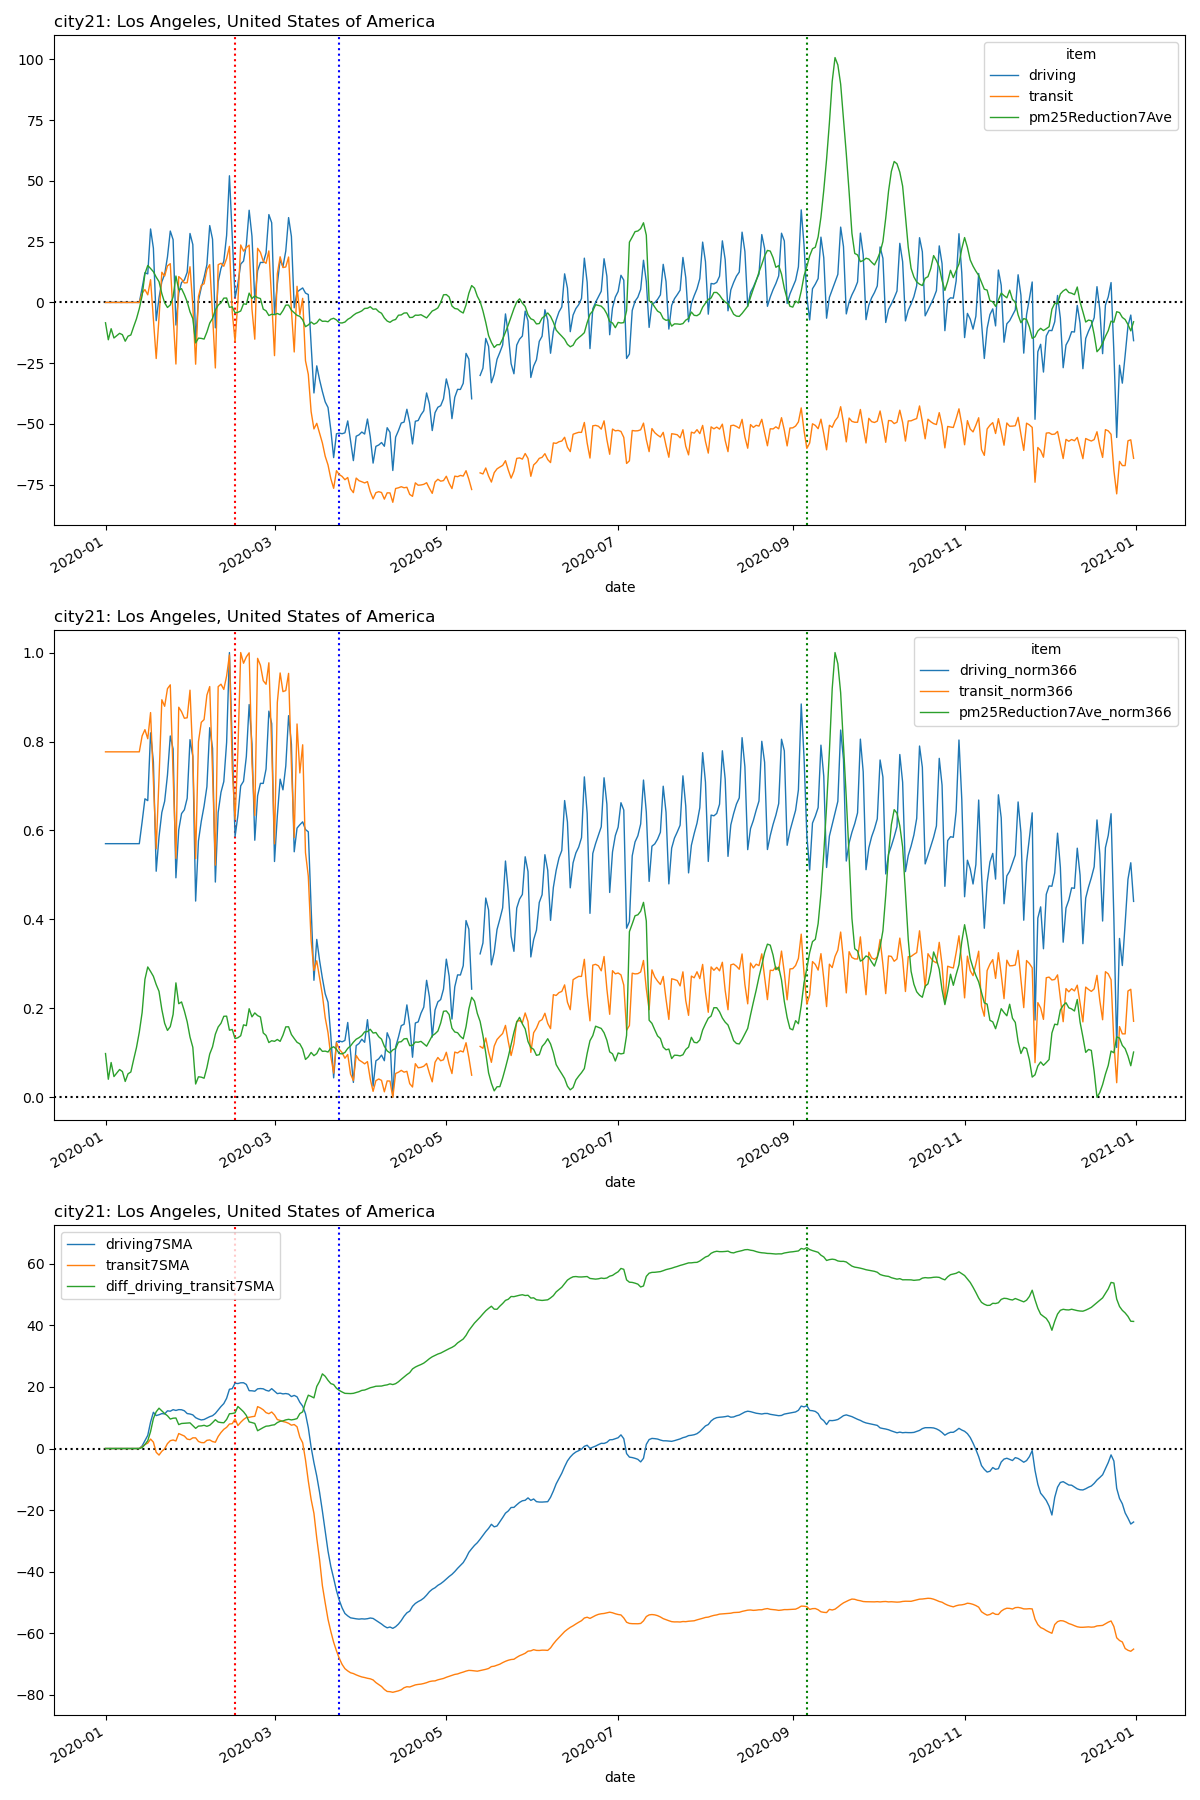
\includegraphics[trim={0 895 0 0},clip,scale=0.45]{Images/LA_Drive_trans.png}
%}
\caption{\bf An overview of the shift in transportation mode preferences during 2020/21, highlighting an increased reliance on private vehicle use over public transit during during the course of the COVID-19 pandemic for the city of Los Angeles, United States of America.}  
 \label{fig:LAdriv_trans}
\end{figure}


\begin{figure}
\centering
%\fbox{
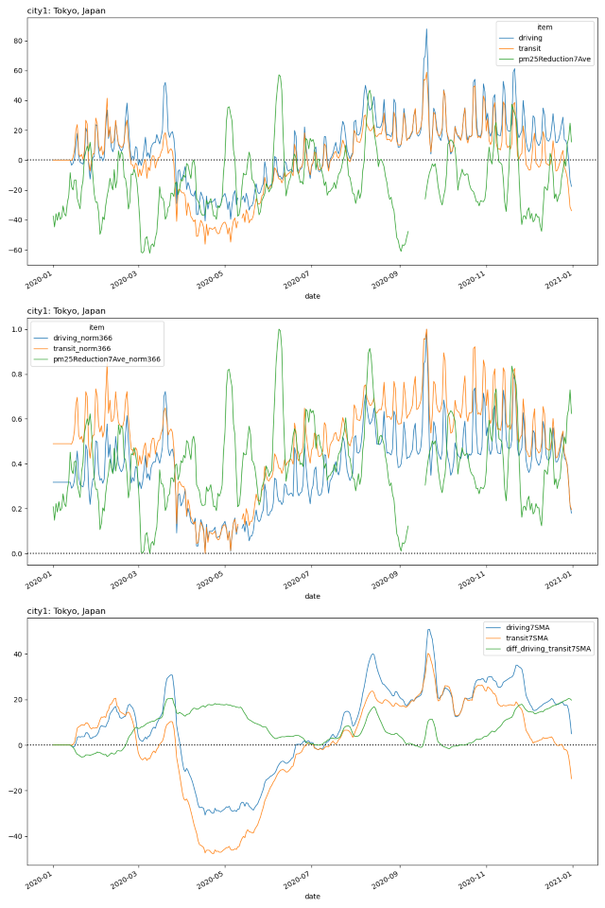
\includegraphics[trim={0 455 0 0},clip,scale=0.9]{Images/TokyoTransit_Driving.png}
%}
\caption{\bf An overview of the shift in transportation mode preferences during 2020/21, highlighting minimal changes to transport model share between public transit and private motor vehicles during during the course of the COVID-19 pandemic for the city of Tokyo, Japan.}  
 \label{fig:TokyoDriv_trans}
\end{figure}


\section*{Discussion}
The underlying structure and design of cities provides a basis upon which citizens move and interact. City designs can afford certain mode choices (e.g., driving or public transit) while constraining others (e.g., walking and cycling). Various patterns of movement and interaction facilitated by city designs translate into either direct (e.g., road crashes) or secondary risk exposures (e.g., exposure to airborne disease or pollution), that can then lead to injury and/or acute and chronic illness, increasing the global burden of disease.

More than half of the worlds greenhouse gas (GHG) emissions have arisen in the period post the United Nations Framework Convention for Climate Change in 1992 \cite{bashmakov2022climate}, with road transport one of the most significant contributors to these emissions. The societal challenge to mitigate GHG emissions by 2030 and net zero by 2050 \cite{lynskey2020moving} is significant, highlighting the urgency to deliver pragmatic solutions now.

Japanese cities are peculiar on the world stage in that they combine a very dense road network with high levels of public transit and almost no on-street parking. This policy shifts responsibility for parking provision onto individual vehicle owners rather than to the public or local government. Therefore, while car-centric city designs afforded populations choices Japanese cities and supporting policies constrain citizens' options to shift between 

The results above demonstrate that optimal city types for health are not static, but change given the health crises and concerns of the time. This should come as no surprise given the role of cities and shared urban infrastructure in historic public health disasters. However, the performance of cities and their role in producing or preventing disease has previously tended to be considered over a period of centuries, decades or years. Here, we demonstrate that optimal designs can also change in acute public health crises that unfold over weeks and months. City designs can facilitate rapid changes in mode-choice which may `stick' for better or worse. 

It therefore follows that the prestige and (ill-)health enjoyed by citizens in even the greatest or `healthiest' of cities or areas is perhaps ephemeral. Times, circumstances, environments, and conditions change that expose citizens to new risks and new public health challenges.


\section*{Conclusion}

\textbf{Funding} States the funding sources.

% \textbf{Notes from Lancet Editor} 
% -	The need to focus on health outcomes. She is particularly interested in ‘hard clinical outcomes’. The journal considers measures of mobility and air pollution as proxy health measures. For example, she would expect to see reduction in asthma in the air pollution paper; 
% -	She agreed a timeline of submission of papers end of March 2023. She emphasised the sooner the better as there will be other papers and series being submitted; 
% -	She is keen to see early drafts and I suggested we would share these in January. I think this is important to get early feedback, particularly around any issues re: appropriateness of health outcomes;
% -	Each paper should be no more than 5000 words;
% -	Need to clearly address why the series of papers is appropriate for The Lancet Public Health (for the cover letter);
% -	How does this series differ from others published, in particular the recent series led by Billie Giles-Corti in The Lancet Global Health (for the cover letter);
% -	Need to include set of recommendations or call to action for series;
% -	Timelines: > 6 months from submission to acceptance (if all goes well).

%Delhi, Bella Horizonte & Belfast





\section*{Contributors}\label{sec:credit}
\textbf{KAN}: Conceptualization, Methodology, Software, Formal Analysis, Writing - Original Draft, Writing - Review \& Editing, Visualization.

\section*{Declaration of interests}\label{sec:dec}
We declare no competing interests.

\section*{Acknowledgments}\label{sec:ak}
KAN is supported by NHMRC/UKRI grant (1194959).


%\section{}
%\label{}

%% The Appendices part is started with the command \appendix;
%% appendix sections are then done as normal sections
%% \appendix

%% \section{}
%% \label{}

%% If you have bibdatabase file and want bibtex to generate the
%% bibitems, please use
%%
%%  \bibliographystyle{elsarticle-num} 
%\bibliography{bibtext.bib}

%% else use the following coding to input the bibitems directly in the
%% TeX file.

\section*{References}\label{sec:ref}
%\begin{thebibliography}{00}

%% \bibitem{label}
%% Text of bibliographic item


\bibliography{bibtext.bib}
\bibliographystyle{elsarticle-num} 
%\bibliography{bib}
\begin{thebibliography}{1}
\expandafter\ifx\csname url\endcsname\relax
  \def\url#1{\texttt{#1}}\fi
\expandafter\ifx\csname urlprefix\endcsname\relax\def\urlprefix{URL }\fi
\expandafter\ifx\csname href\endcsname\relax
  \def\href#1#2{#2} \def\path#1{#1}\fi

\end{thebibliography}
\end{document}
\endinput
%%
%% End of file `elsarticle-template-num.tex'.


